\documentclass{article}

\usepackage{graphicx}

\usepackage[margin=0.5cm]{geometry}
\usepackage{amsmath}
\usepackage{indentfirst}
\usepackage{hyperref}
\usepackage{multirow}
\usepackage{comment}

\newcommand{\cosa}{\cos\hat\alpha}
\newcommand{\size}{0.33\textwidth}

\begin{document}

\clearpage

\newgeometry{margin = 0.5cm}

\begin{figure}[h!]
\centering
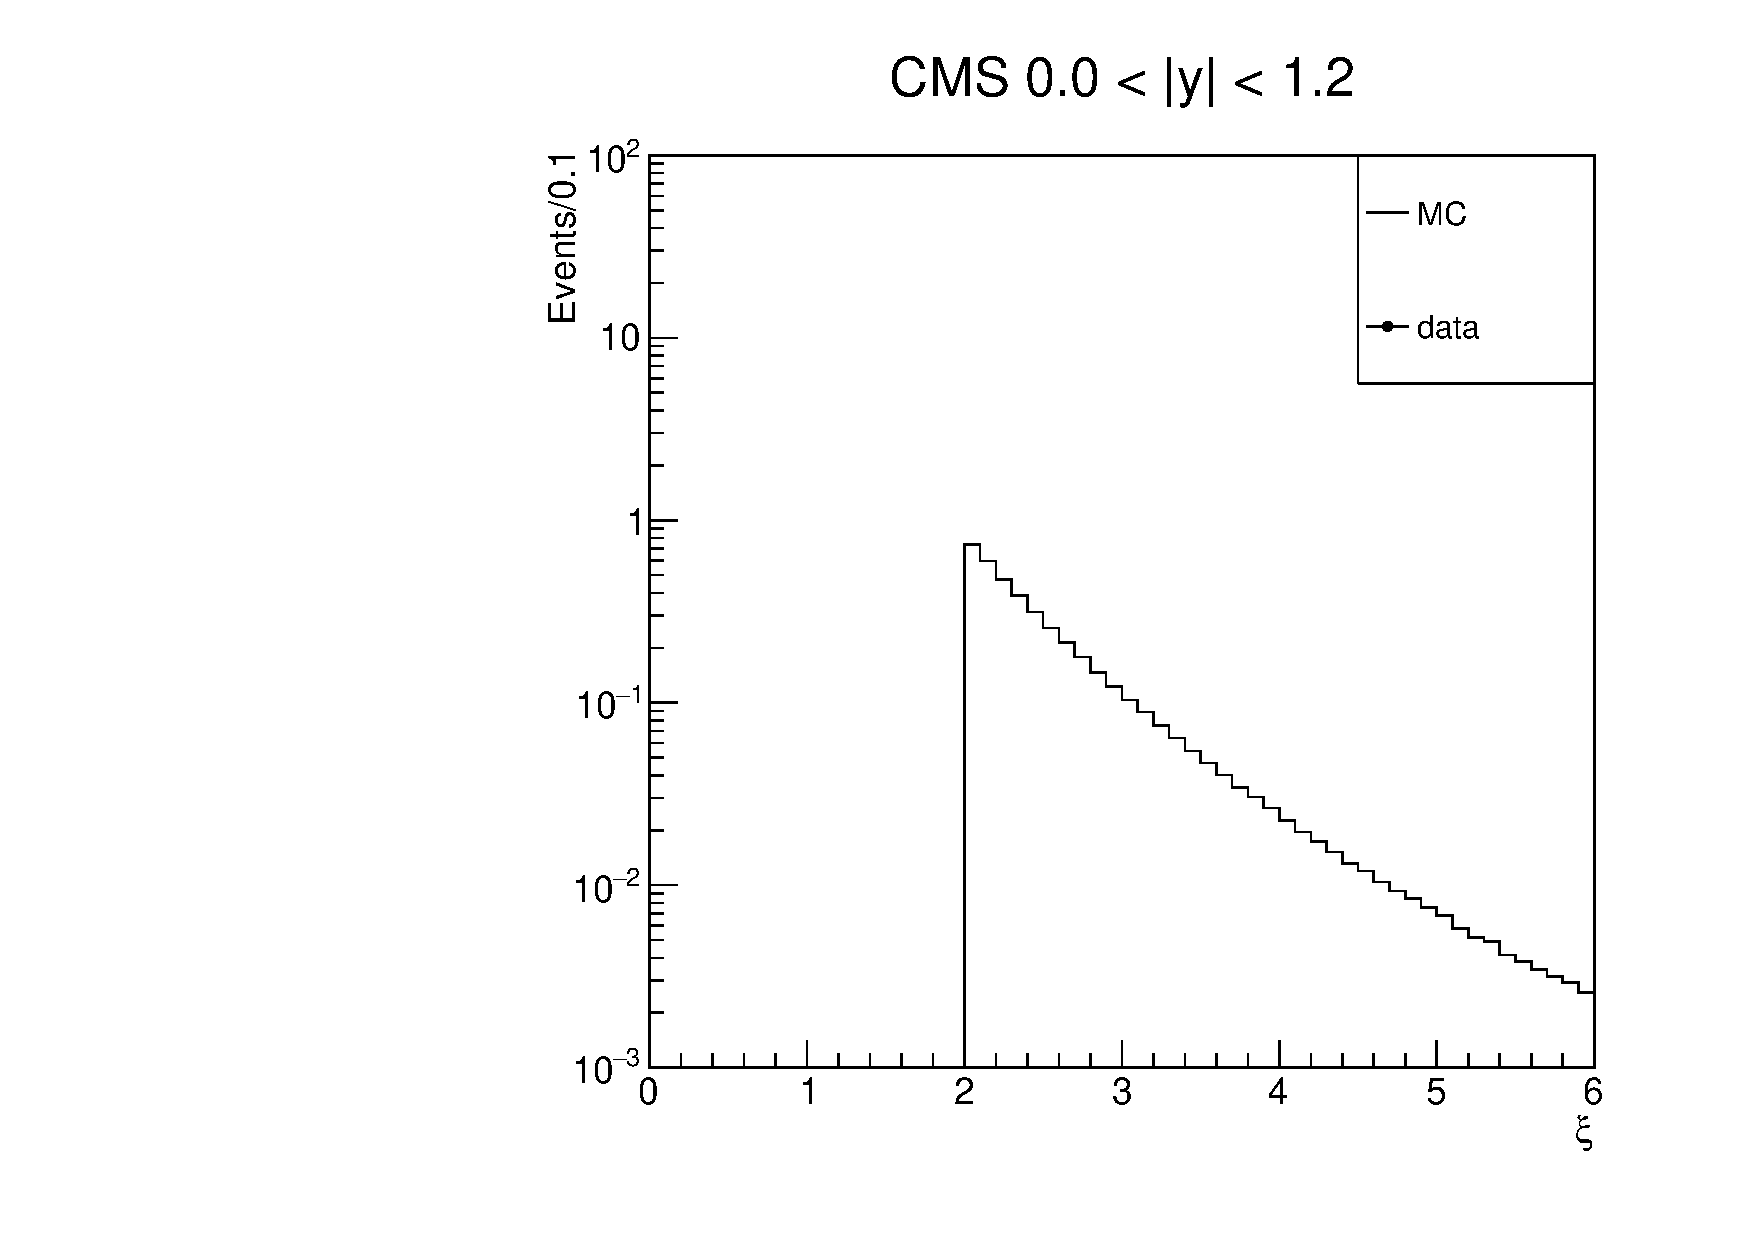
\includegraphics[width = 0.4\textwidth]{plots/xi_CMS.pdf}
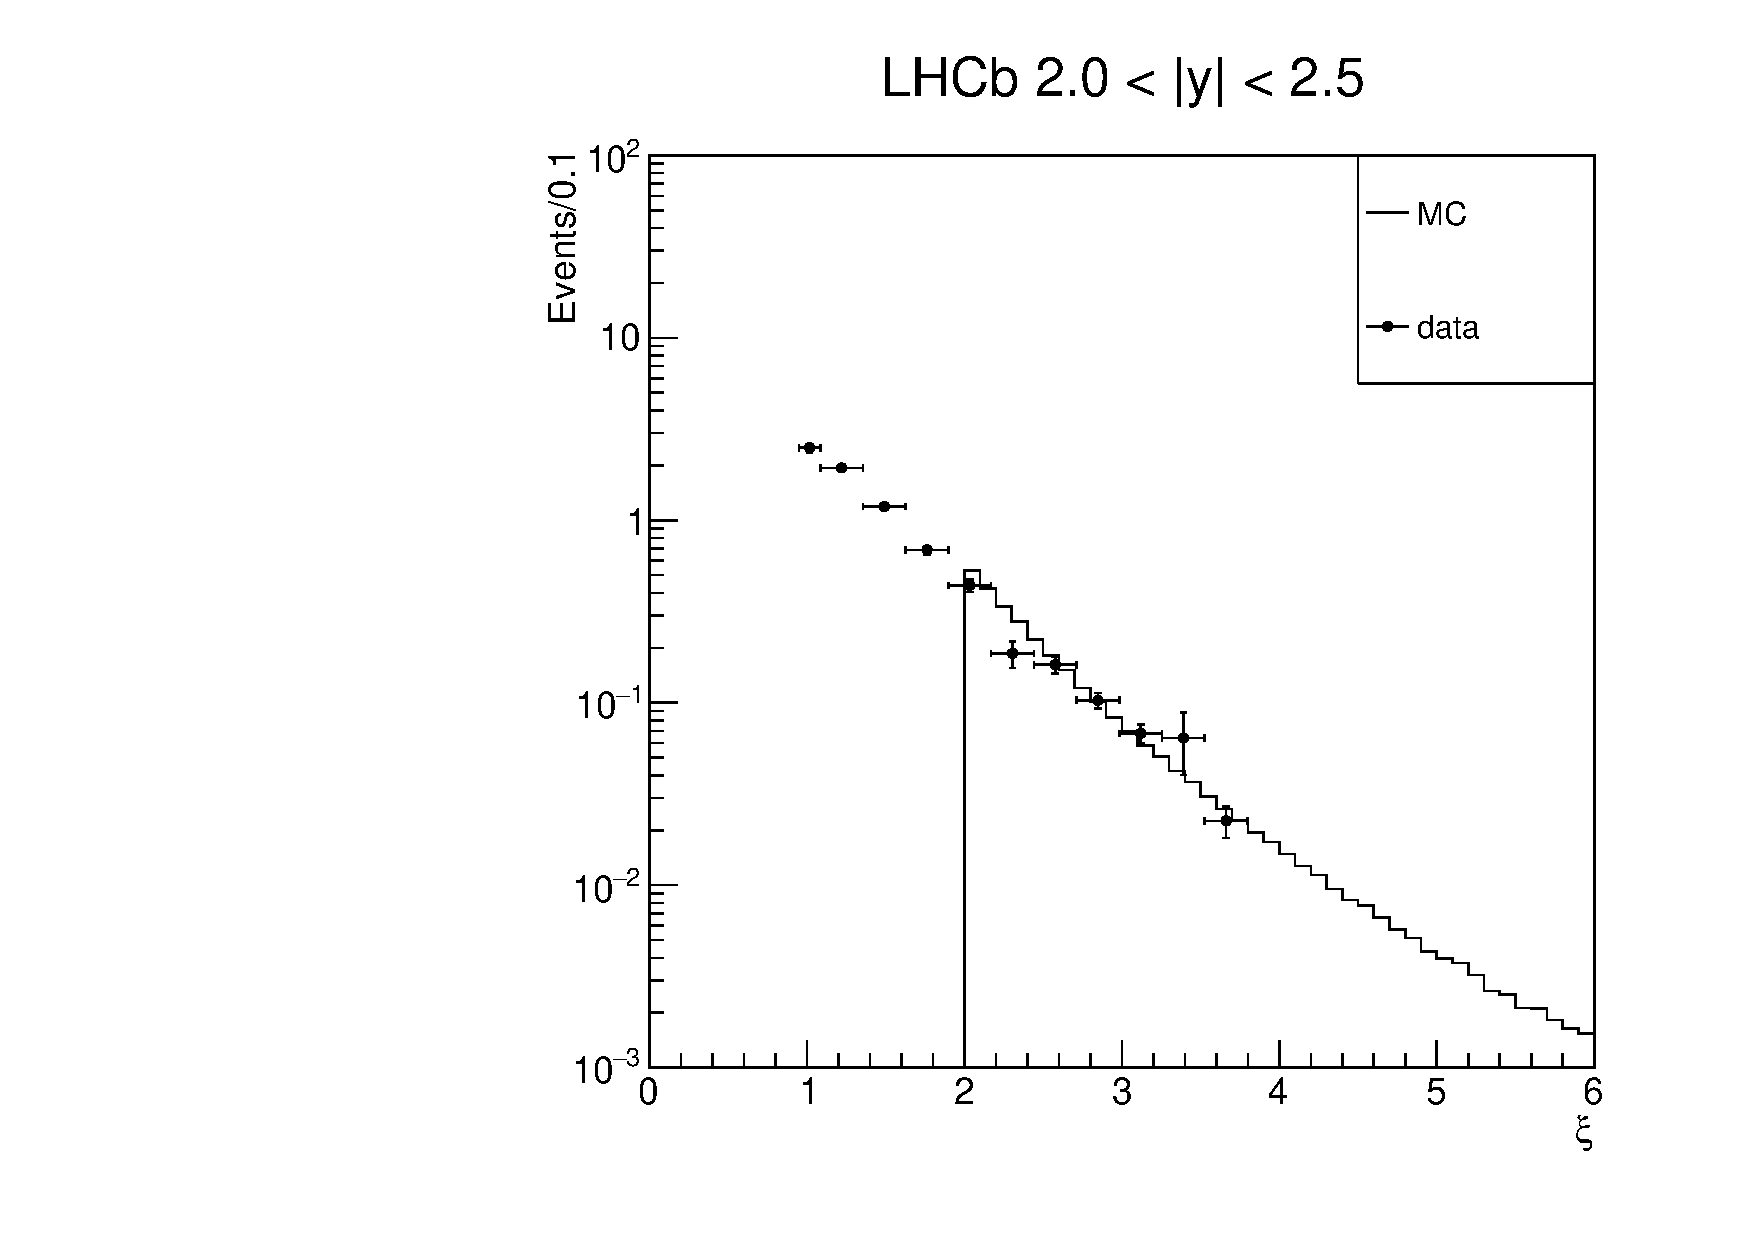
\includegraphics[width = 0.4\textwidth]{plots/xi_LHCb_y1.pdf}

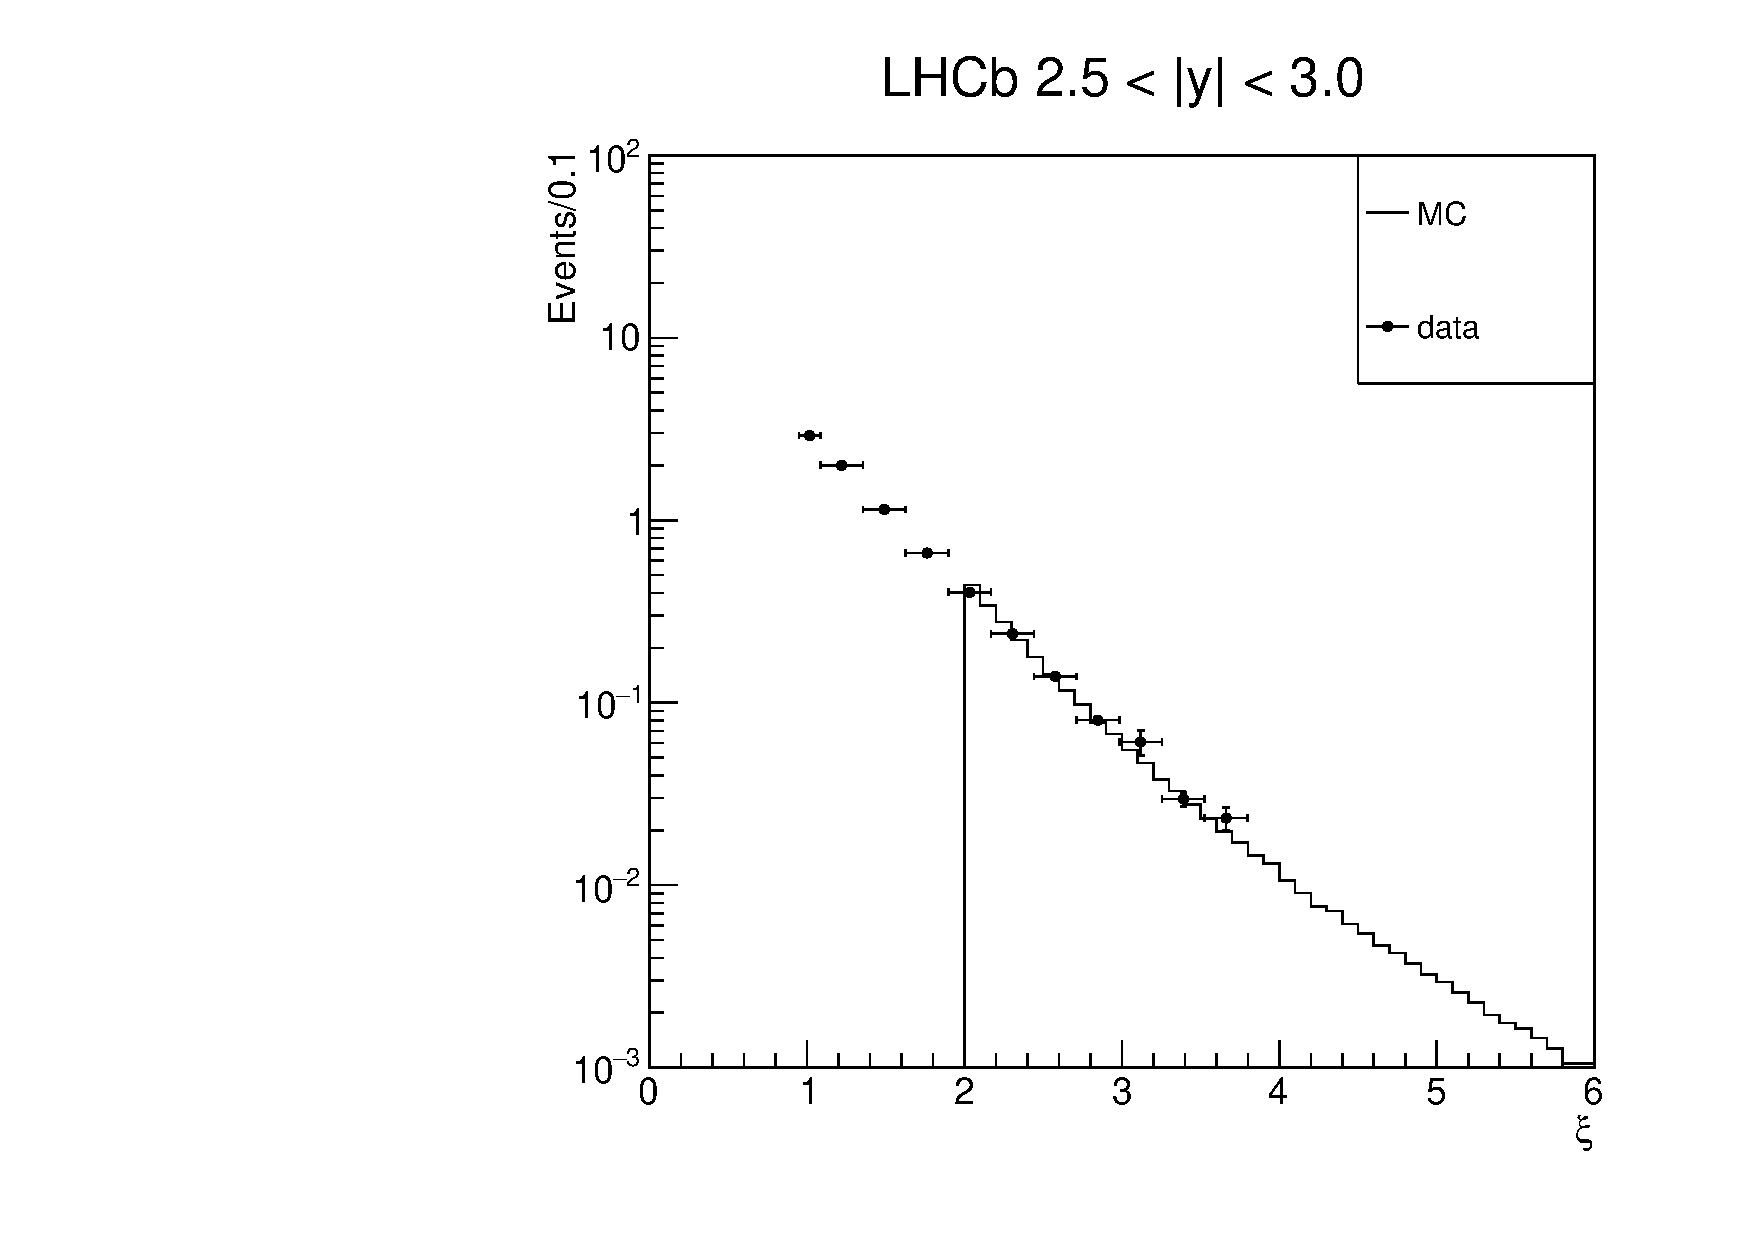
\includegraphics[width = 0.4\textwidth]{plots/xi_LHCb_y2.pdf}
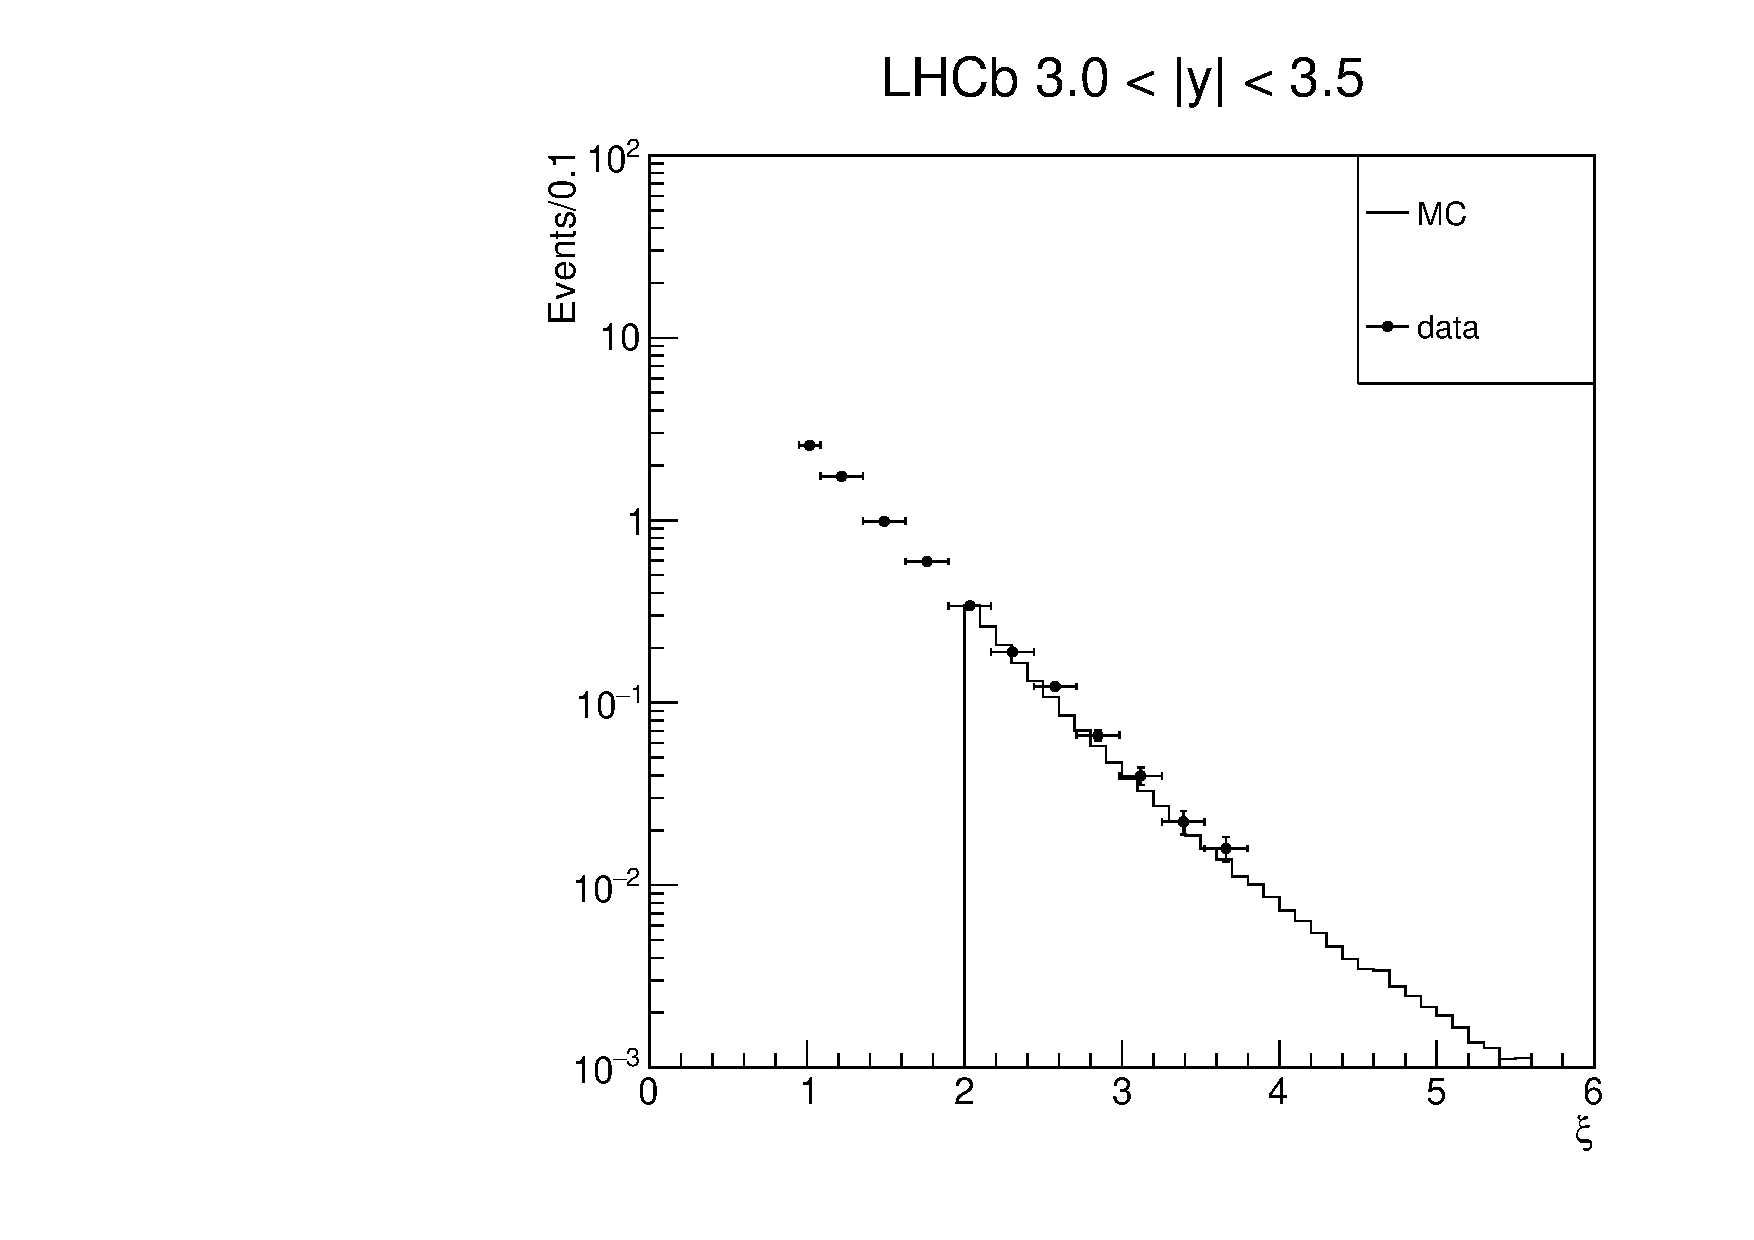
\includegraphics[width = 0.4\textwidth]{plots/xi_LHCb_y3.pdf}

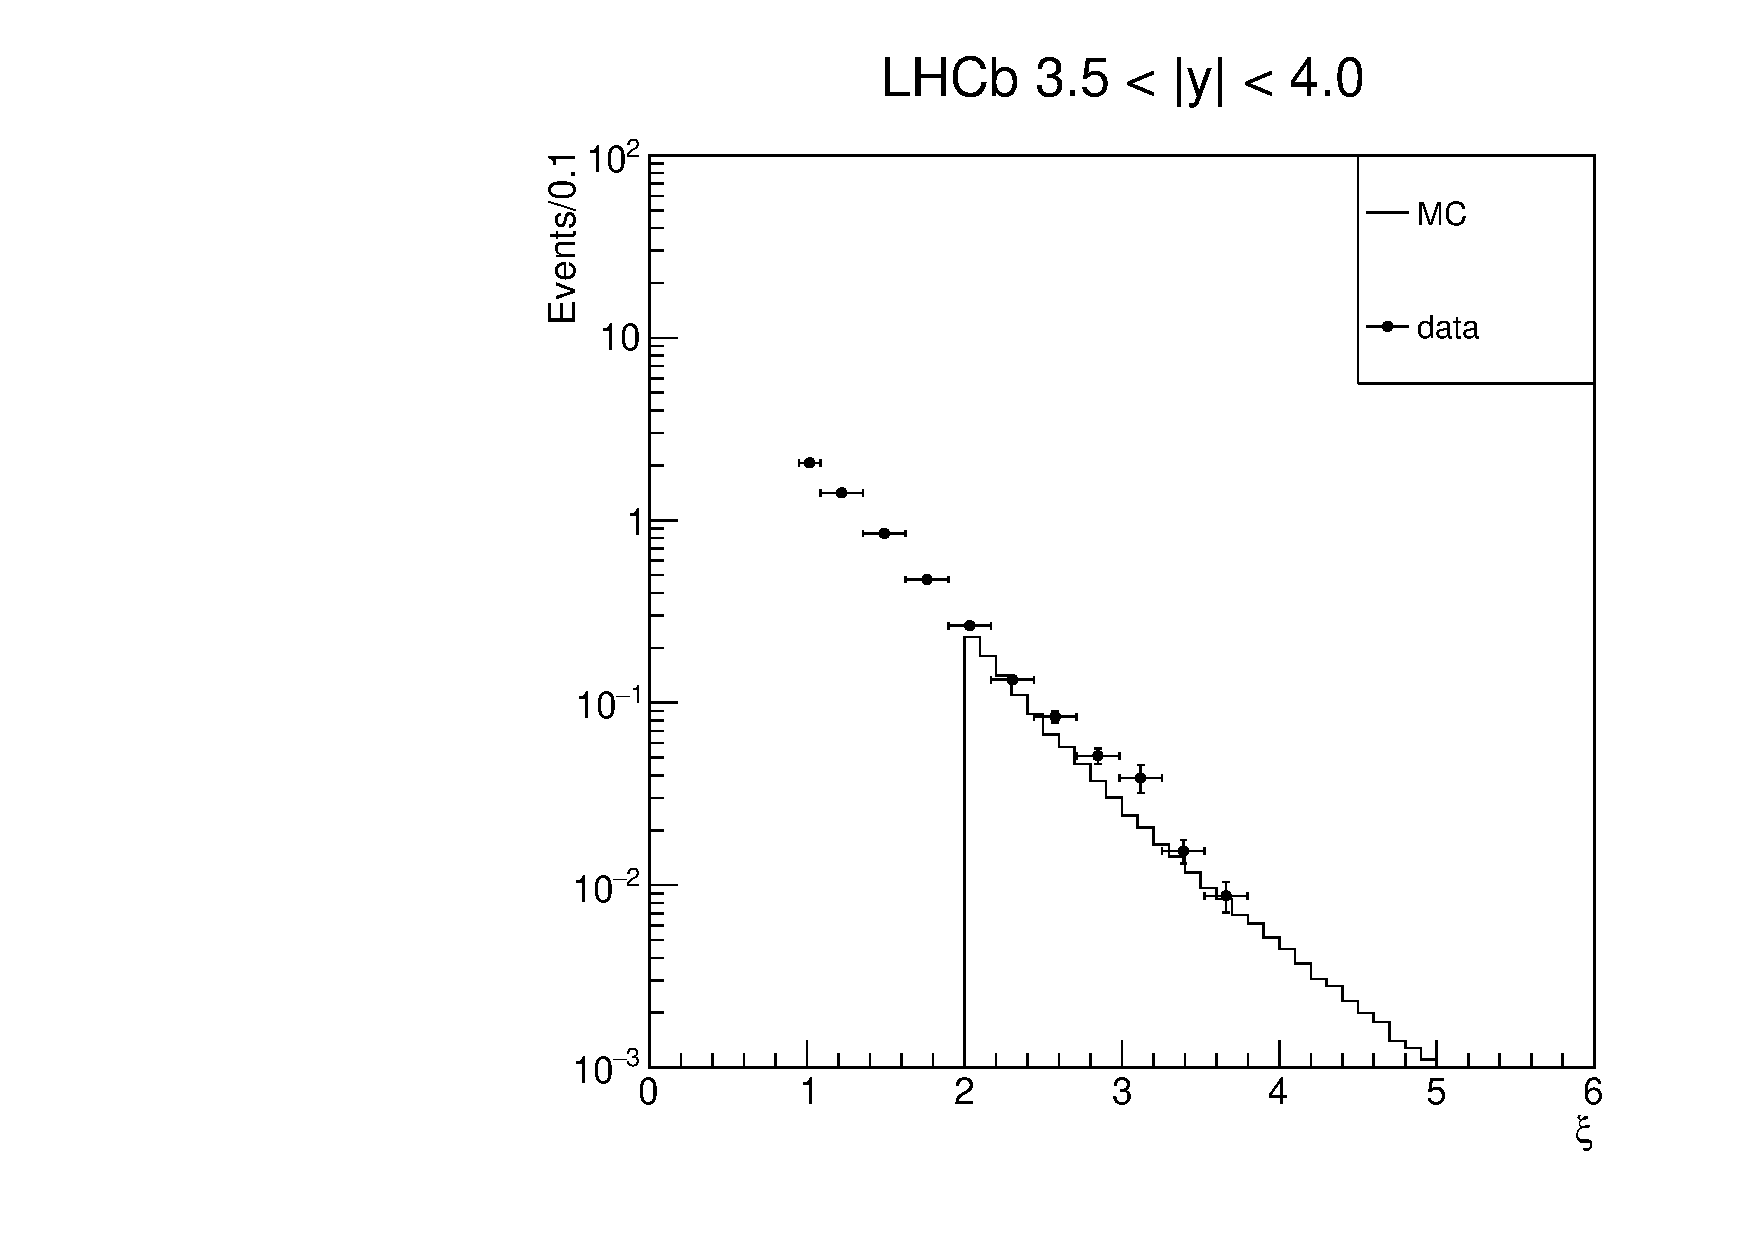
\includegraphics[width = 0.4\textwidth]{plots/xi_LHCb_y4.pdf}
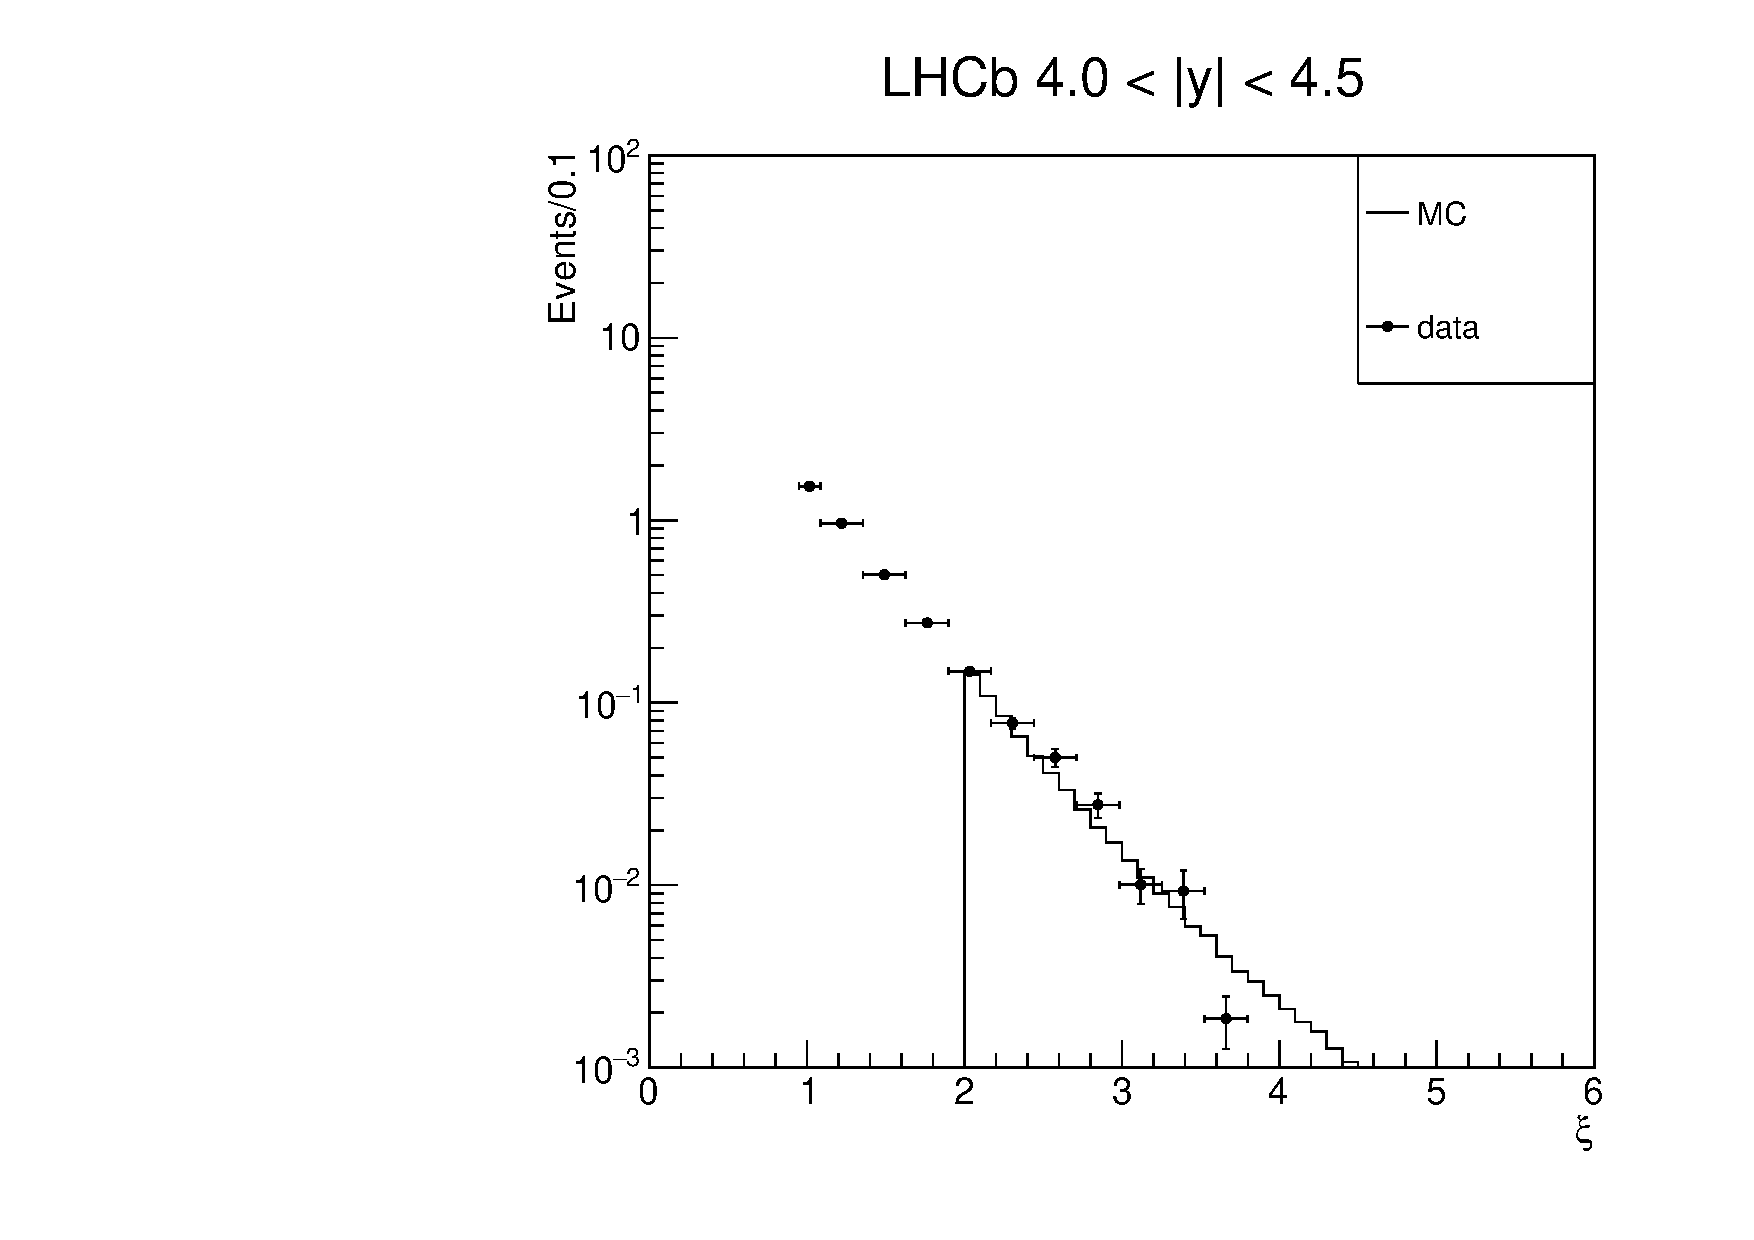
\includegraphics[width = 0.4\textwidth]{plots/xi_LHCb_y5.pdf}
\caption{Comparison between MC $\xi$ distribution and data points for new sample in each of the $y$ bins of the data. MC distributions scaled by the integral of the $|y|<1.2$ distribution. Data points scaled by the value of the first CMS data point $\times 10$.}\label{f:xi_comp_new}
\end{figure}

\clearpage

\begin{figure}[h!]
\centering
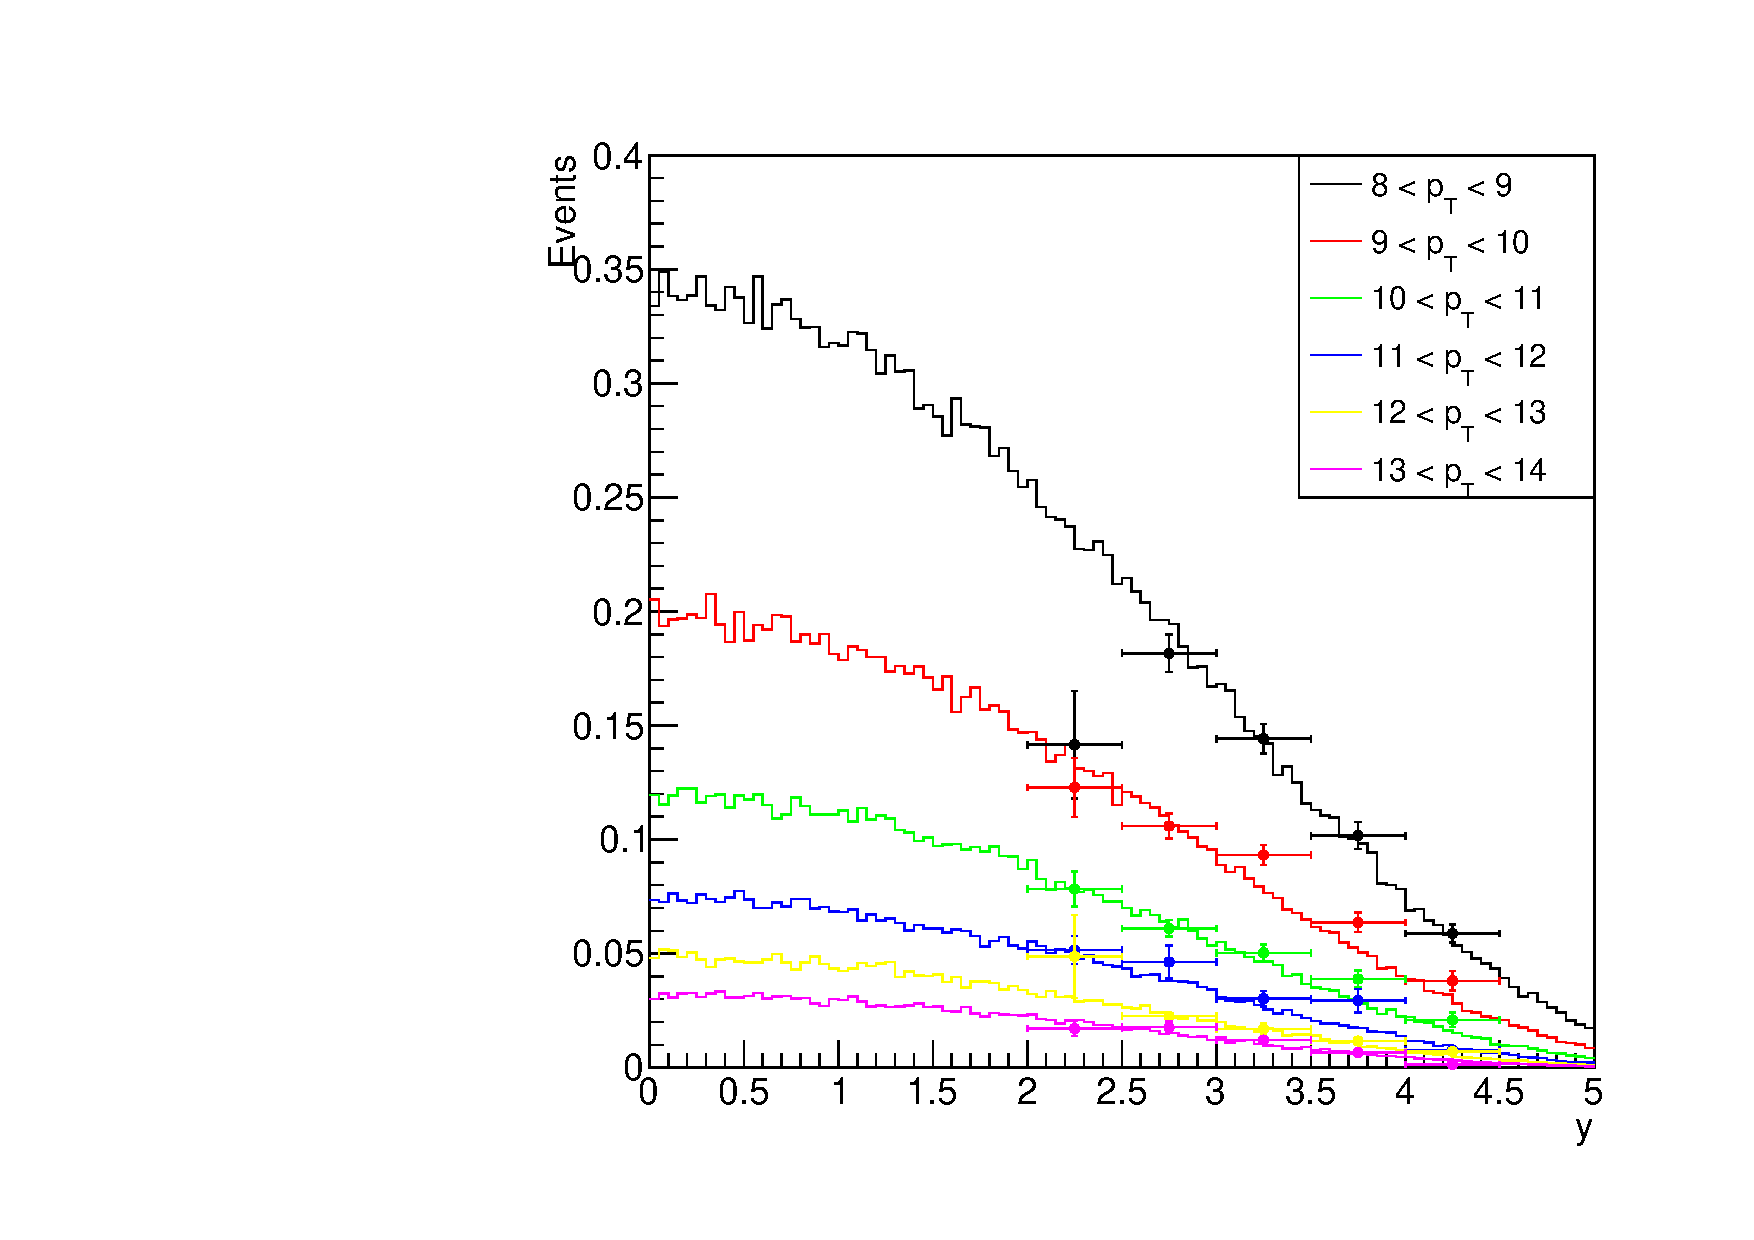
\includegraphics[width = 0.4\textwidth]{plots/y_dist.pdf}

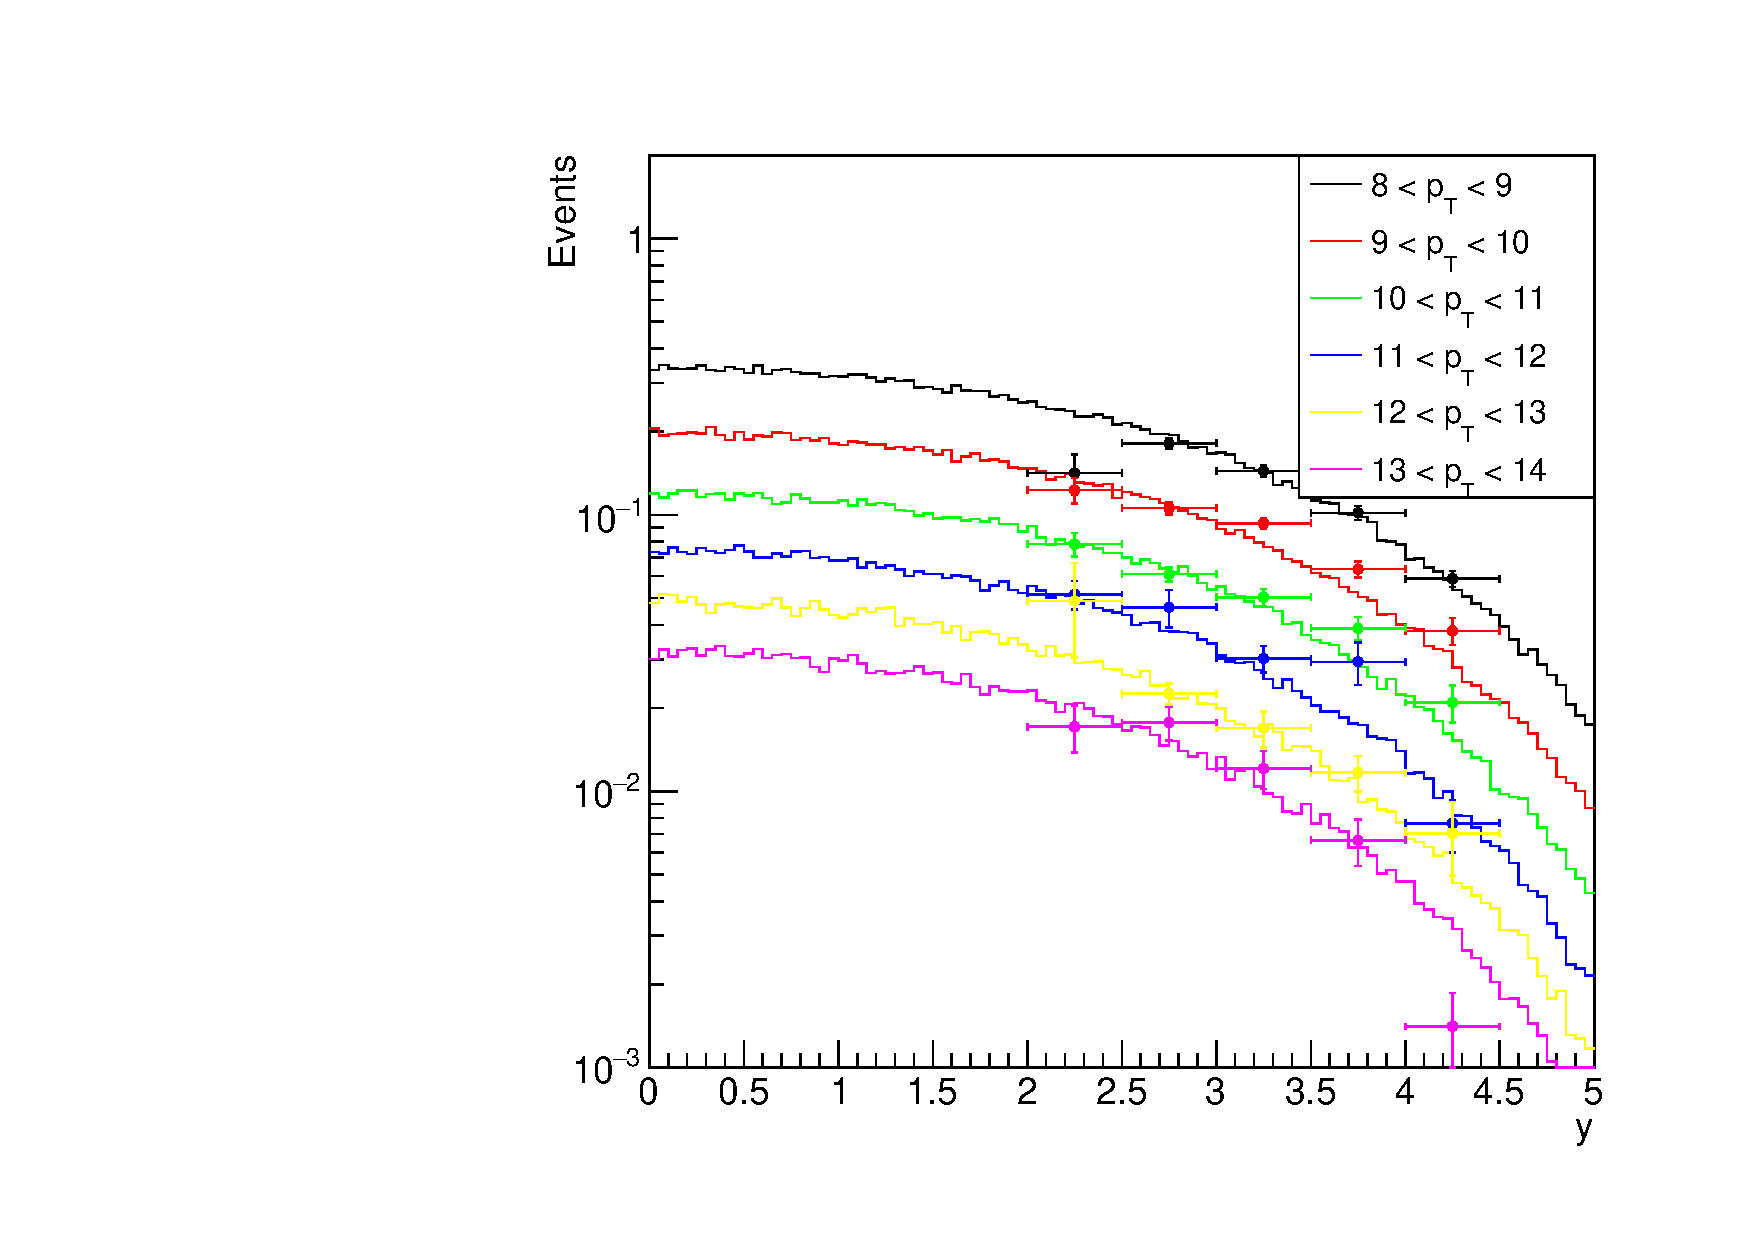
\includegraphics[width = 0.4\textwidth]{plots/y_dist_log.pdf}
\caption{MC $y$ distributions, lin- (top) and log-scale (bottom) in each of the 1 GeV-wide $p_\text T$ bins of the data. MC distributions scaled by the integral of the $7<p_\text{T}<8$ distribution.}\label{f:y_comp_rho_log}
\end{figure}

\end{document}